%%%%%%%%%%%%%%%%%%%%%%%%%%%%%%%%%%%%%%%%%%%%%%%%%%%%
% This will help you in writing your homebook
% Remember that the character % is a comment in latex
%
% chapter 2
\chapter{Testbench}
\label{cha2}

%% To verify if the multiplier works correctly a testbench is needed.

\section{Design modification}
Before to proceed with the simulation some modifications have been added to improve
the testability:
\begin{itemize}
    \item Add registers to inputs and a reset signal, to achieve a better behavior;
    \item Add a VIN and VOUT signals that have the purpose to start the operation
        and to say when it's over.
\end{itemize}

\section{Simulation}
The testbench has been divided in three parts.
\begin{itemize}
    \item The first part generates inputs that will feed the multiplier, that will be the element under test (DUT). Those 
    inputs will be taken from an input file that has been generated thanks to C prototype, like explain int the previous chapter.
    The same input feed both factor and the VIN signal will be keep high until all input values have been used.
    \item When outputs start to be ready VOUT signal will be raised and, until this signal is high, a text file 
    will be written in order to see which will be the produced results. Then those values will be compared with 
    golden ones, that have been generated from C prototype script, to check the correctness of multiplier. 
    \item The last part generates the clock that will feed the input generator, the data sink and the DUT.
\end{itemize}

\begin{figure}[!htb]
    \begin{minipage}{0.48\textwidth}
      \centering
      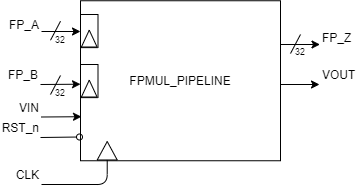
\includegraphics[width=.8\linewidth]{ {./schematic/FPmul_schematic.png} }
      \caption{}\label{Fig:a}
    \end{minipage}\hfill
    \begin{minipage}{0.48\textwidth}
      \centering
      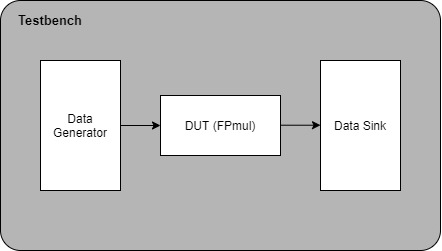
\includegraphics[width=.8\linewidth]{ {./schematic/testbench} }
      \caption{}\label{Fig:b}
    \end{minipage}
 \end{figure}